\subsection{Raster datamodel} \label{Afsnit: Raster data model}

En rastermodel er en datamodel der er bygget op af et regulært netværk af celler organiseret i et gitterformat \citep{bolstad_gis_2022, esri_raster}. Hver celle i en raster model er karakteriseret af en celle dimension, som definerer cellestørrelsen ud fra cellens længde i X- og Y-retningen \citep{bolstad_gis_2022}. Cellestørrelsen repræsenterer således den rumlige opløsning af raster datamodellen og fungerer som en indikator for datasættets rumlige præcision, da hver celles koordinat er givet ud fra centrum af cellen. En større cellestørrelse vil derfor resultere i en højere rumlig usikkerhed, mens en mindre cellestørrelse vil medføre en lavere rumlig usikkerhed. En mindre cellestørrelse medfører også et større datasæt og optager mere plads i databaser \citep{bolstad_gis_2022}. Rastermodellen er derfor en afvejning af god opløsning og minimering af  filstørrelsen.\\

Hver celle i en raster indeholder en værdi, der repræsenterer information om det pågældende geografiske område. Disse værdier kan enten være numeriske eller kategoriske, afhængigt af den type data, der ønskes repræsenteret. Numeriske værdier anvendes typisk til at beskrive kontinuerlige data, hvor værdierne kan variere gradvist fra celle til celle. Et eksempel på dette er højdemodeller, hvor hver celle indeholder en talværdi, der angiver terrænets højde (figur \ref{Subfig: Kontinuer raster}). Andre eksempler på kontinuerlige rasterdata er temperatur, nedbør eller koncentration af et bestemt stof i jorden. \\
Kategoriske værdier bruges derimod til at repræsentere diskrete eller tematiske værdier, hvor hver celle tildeles en bestemt kategori eller klasse. Dette ses fx i arealanvendelses datasæt, hvor hver celle angiver om området er dækket af skov eller en bestemt trætype (figur \ref{Subfig: Kategorisk raster}).
\begin{figure}[H]
    \begin{subfigure} [t]{0.5\textwidth}
        \centering
        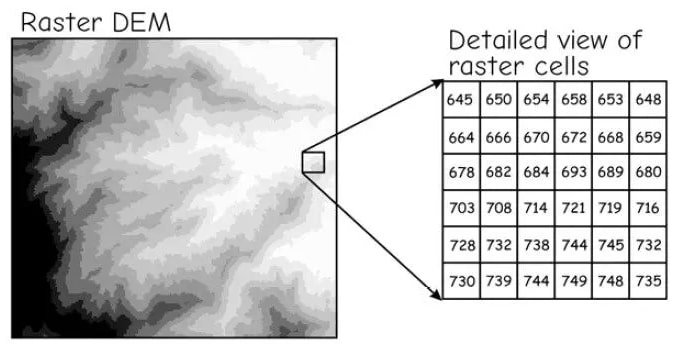
\includegraphics[width=1\linewidth]{images/teori/raster_kontinuert.jpg}
        \caption{}
        \label{Subfig: Kontinuer raster}
    \end{subfigure}
    \begin{subfigure} [t]{0.5\textwidth}
        \centering
        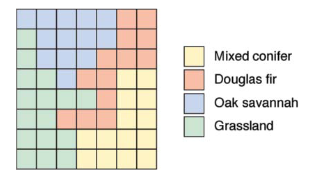
\includegraphics[width=1\linewidth]{images/teori/raster_areal.png}
        \caption{}
        \label{Subfig: Kategorisk raster}
    \end{subfigure}
    \caption{Eksmepler på to forskellige typer af information lagret i en raster datamodel. \textbf{(a)} Numerisk og kontinuert data fra en højdemodel. \textbf{(b)} Kategorisk raster med diskrete data over forskellige trætyper og arealanvendelser. Kilde: \cite[s. 66]{bolstad_gis_2022} og \cite[s. 67]{longley_geographical_2008}.}
    \label{Figur: Kontinuert og kategorisk raster}
\end{figure}
Det er vigtigt at bemærke at rasterceller også kan indeholde en unik værdi, der angiver "NoData", hvis der ikke foreligger information for den pågældende celle. NoData værdier gør det muligt at både kunne håndtere ufuldstændige datasæt og sikre at analyser kun udføres på relevante celler \citep{bolstad_gis_2022, longley_geographical_2008}. NoData-celler kan indgå i logiske og betingende udtryk i rasterberegninger, hvor NoData-celler kan identificeres. Det skal derimod understreges at aritmetiske operationer ikke kan udføres på celler med NoData. Alle numeriske beregninger med NoData vil altid resultere i NoData. Denne egenskab kan ændres ved at sætte alle NoData værdier i et rasterdatasæt til den samme værdi, fx 0 eller 999 \citep{bolstad_gis_2022}.\\

Rastermodellens struktur muliggør derfor omfattende rumlig analyse, idet der kan udføres aritmetiske og logiske operationer på tværs af celler og mellem flere forskellige typer af rastere. Denne egenskab gør det derfor muligt at analysere og kombinere kontinuerte og diskrete rumlige informationer i et GIS-miljø \citep{bolstad_gis_2022, longley_geographical_2008}. Det er også muligt at udføre analyse med andre datatyper såsom mellem raster og vektordata. Analyser der kombinerer begge datatyper gør det er det muligt at lave kombineret vektor- og raster modeller i et GIS-miljø der kan bruges til at lave stormflodsmodellering.

\subsection{Inundation Modellen} \label{Afsnit: Inundation Model}

Til at lave stormflodsmodelleringen i dette projekt, er der blevet anvendt en GIS-baseret screeningsmodel til stormfloder,  \textit{"Inundation Model"} udarbejdet af \cite{balstrom_kirby_inundation} til at give et bud på hvordan en stormflod vil påvirke et område. Modellen opererer eksklusivt i et ArcGIS Pro miljø, GIS-softwaren udviklet af Esri. I dette afsnit vil der blive redegjort for den tekniske del af hvordan modellen fungerer.\\

Modellen indeholder en række værktøjer, der bruges til at analysere stormfloders påvirkning af et område og kernen i modellen er værktøjet \textit{"Create Inundation"}, en statisk numerisk rastermodel. Det er dette værktøj der laver beregningen af hvordan en stormflod vil påvirke et område.\\ 
Modellen tager tre brugerdefineret parametre der består af tre numeriske værdier i meter som input: InitialSealLevel, SeaLevelIncrement og Number of Iterations. InitialSeaLevel bruges som en startværdi for modellen til at itererer over. SeaLevelIncrement er den værdi modellen skal stige med efter hver iteration (fx 1 cm stigning). Number of Iterations er antallet af gentagelser modellen udører. \\
Modellen benytter en hydrologisk korrigeret digital terrænmodel (DHyM) og et digitaliseret linjeobjekt som kilde for udregningen, benævt i modellen som Line at Sea \citep{balstrom_kirby_inundation}. I figur \ref{Figur: Create Inundation} er modellens struktur vist inddelt i to dele.
\begin{figure}[H]
    \centering
    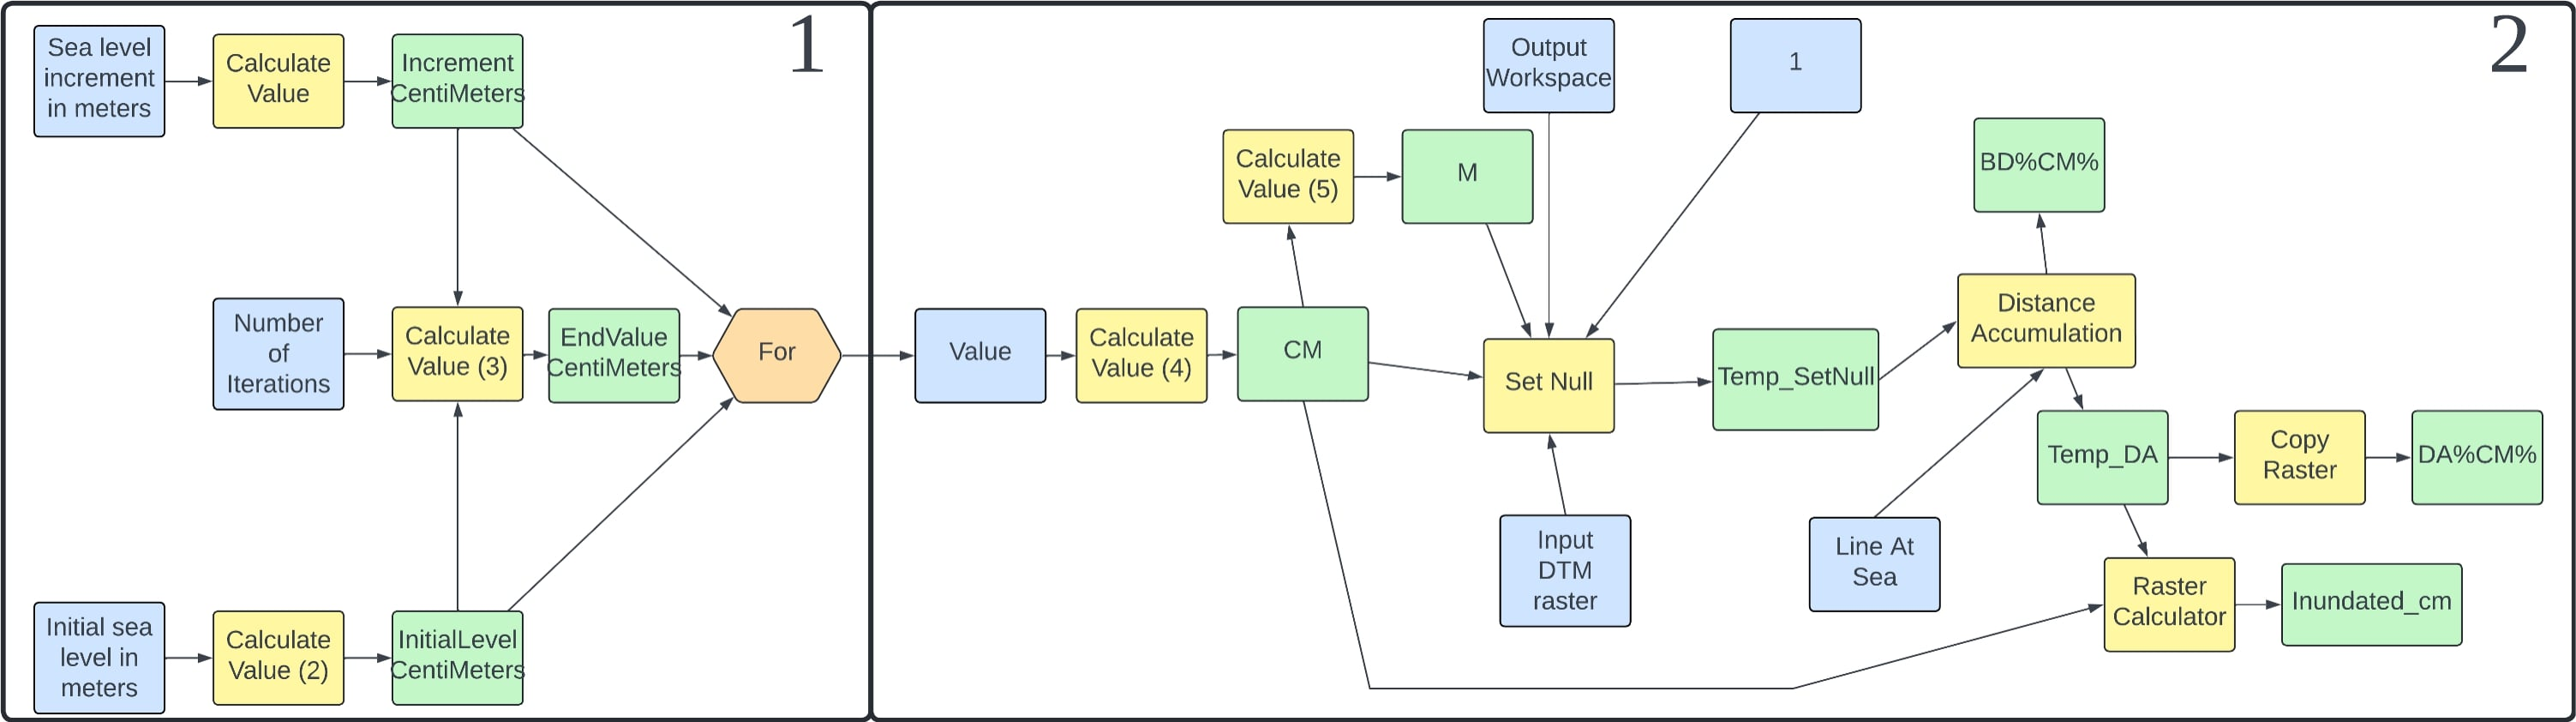
\includegraphics[width=1\linewidth]{images/teori/inundation_model_separated.jpg}
    \caption{Flowchart af Inundation Modellens \textit{"Create Inundation"} værktøj.}
    \label{Figur: Create Inundation}
\end{figure}
Den første del er en omregning af brugerens input fra meter til centimeter for både stigningsniveauet for hver gang modellen itererer og det begyndende havniveau. Modellen kræver en afsluttende værdi for hvornår den skal stoppe med at iterere, som svarer til den vandstand der ønskes at simuleres op til. Denne værdi bliver udregnet ved følgende: \\$InitialSeaLevel + ((NumberIterations - 1)\times Increment)$. På samme vis kan en omvendt udregning laves for at finde antallet af gentagelser for at opnå en bestemt vandstand. Dette gøres ved: $(EndValue - InitialSeaLevel) / Increment - 1$. Dette tillader brugeren at simulere en stormflod til en ønsket vandstand.\\

Den anden del af modellen er selve beregningen af stormflodens oversvømmelse igennem terrænmodellen. Det starter med et for-loop der starter med den første værdi (fx 100 cm). Denne værdi omregnes tilbage til meter hvorefter modellen eksekverer et hvis-ellers tjek (figur \ref{Figur: Create Inundation} \textit{"SetNull"}) på cellerne i DTM. Her tjekkes alle celleværdierne i DTM for om de er større eller ligmed den værdi der tjekkes for. Hvis dette hvis-ellers tjek er sandt, hvis værdien i DTM er højere end tjekværdien, bliver cellerne tildelt NoData værdien, som indikerer at cellen ikke bliver oversvømmet ved dette vandstandsniveau. Hvis DTM celleværdien er lavere end tjekværdien og udtrykket dermed er falsk bliver cellen angivet med et 1, som indikerer at cellen oversvømmes ved det niveau. I figur \ref{Subfig: Celler Inundated} er der vist hvordan det sker for tre iterationer startende på 100 cm med en stigning på 10 cm. Her det værd at nævne at hver celle der tjekkes for ikke udelukker hinanden, så den næste værdi (110 cm) vil også tildele et 1 til de samme celler, som den foregående værdi. 
\begin{figure}[H]
    \begin{subfigure}[t]{0.5\textwidth}
        \centering
        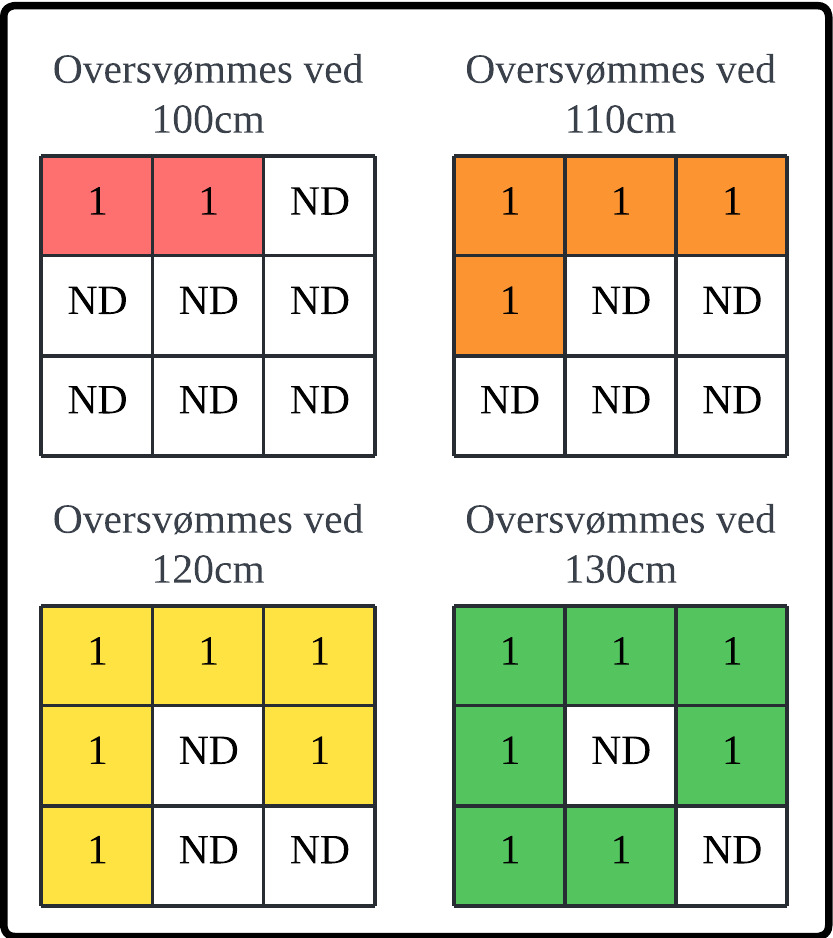
\includegraphics[width=0.7\linewidth]{images/teori/inundated_cells.jpeg}
        \caption{}
        \label{Subfig: Celler Inundated}
    \end{subfigure}
    \begin{subfigure}[t]{0.5\textwidth}
        \centering
        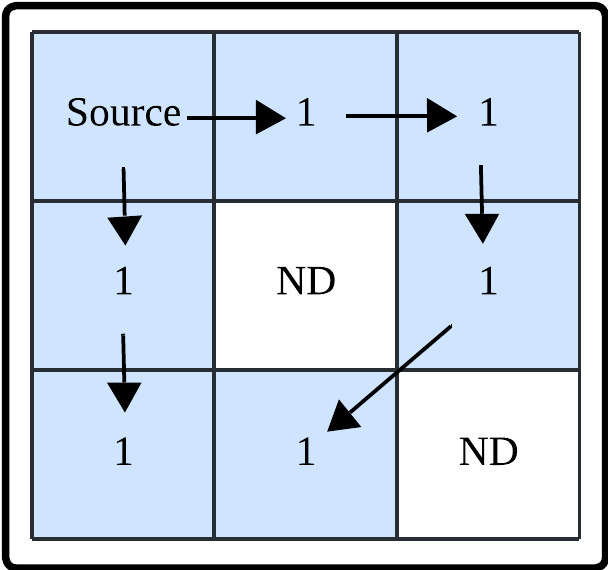
\includegraphics[width=0.85\linewidth]{images/teori/distance_accumulation.jpeg}
        \caption{}
        \label{Subfig: DA}
    \end{subfigure}
    \caption{Principperne bag Inundation Modellen. 1 = Celler der kan oversvømmes, ND = NoData (celler som ikke kan oversvømmes). \textbf{(a)} SetNull funktionen der bestemmer hvilke celler der kan oversvømmes ved et pågældende vandstandsniveau. \textbf{(b)} Distance-Accumulation fra et startpunkt (source) gennem passerbare celler for det pågældende vandstandsniveau. Kilde: Egen illustration med inspiration fra \cite{balstrom_kirby_inundation}.}
    \label{Figur: }
\end{figure}
%\begin{figure}[H]
 %   \centering
 %   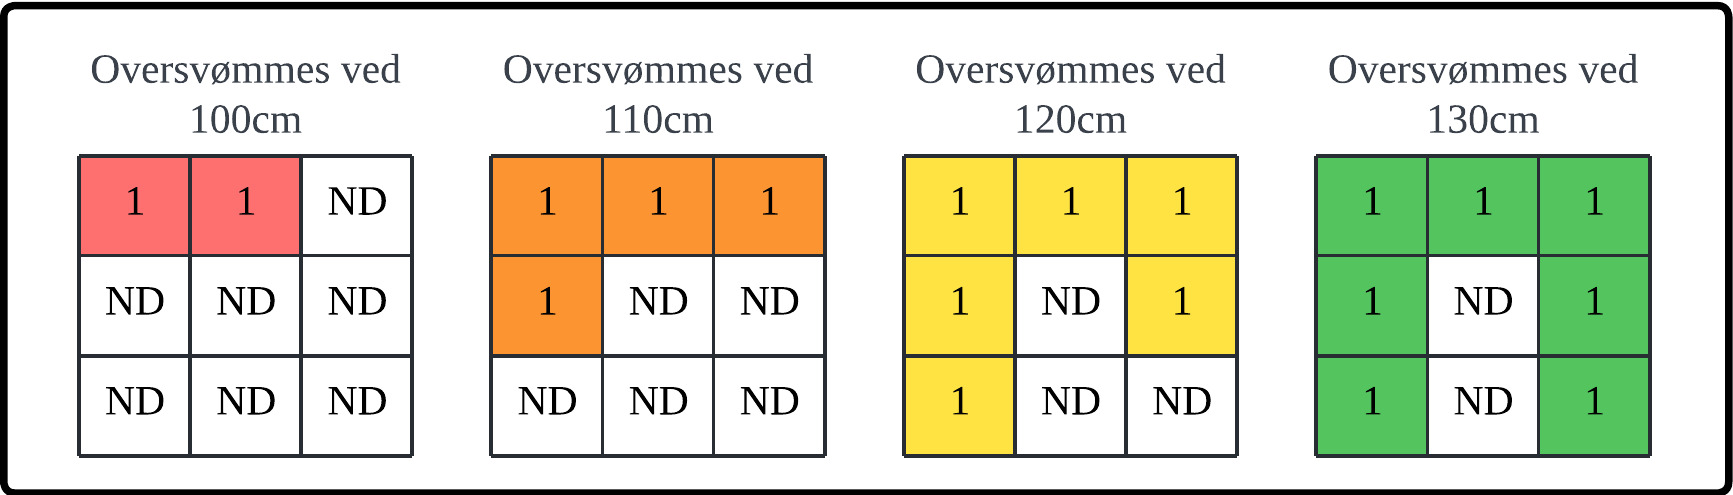
\includegraphics[width=0.8\linewidth]{images/teori/celler_inundated.jpeg}
  %  \caption{Princippet bag Inundation Modellens SetNull funktion gennem cellerne i en højdemodel. 1 angiver at cellen oversvømmes ved det pågældende niveau og ND = NoData (celler som ikke bliver oversvømmet). Egen illustration med inspiration fra \cite{balstrom_kirby_inundation}.}
  %  \label{Figur: Celler Inundated}
%\end{figure}
Herefter gennemføres en Distance Accumulation-analyse igennem de celler der bliver oversvømmet, ved det bestemte niveau, fra linjekilden Line at Sea. En Distance Accumulation er en analysemetode der beregner den samlede afstand fra en defineret kilde ud igennem cellerne i en raster \citep{esri_how_nodate}. I Inundation modellen bliver Distance Accumulation brugt til at efterligne vandets bevægelse igennem cellerne på samme måde som vandet ville sprede sig i gennem terrænet under en stormflod. Distance Accumulation forsætter gennem cellerne, indtil der rammes en uigennemtrængelig barriere (figur \ref{Subfig: DA}). Til at sprede sig igennem cellerne bruges der en "eight-side" \hspace{0.2cm}regel, der er med til at bestemme hvilke celler der kan spredes til. Eight-side reglen fortæller Distance Accumulation værktøjet at der skal tjekkes for en passerbar celle i otte retninger fra en celle.\\

I Inundation Modellen starter Distance Accumulation fra et punkt på linjen \textit{"Line at Sea"} markeret med \textit{"Source"} i figur \ref{Subfig: DA}, og bevæger sig igennem alle cellerne i terrænet hvor cellen = 1. Hvis cellen er NoData så kan vandet ikke bevæge sig igennem \citep{balstrom_kirby_inundation}. Resultatet af Distance Accumulationen bliver derefter koblet med det oversvømmelsesniveau der bliver itereret over for at give resultatet af modellen. Resultatet lagres som en raster og der lagres en raster for hver værdi der itereres over. Processen starter derefter forfra indtil simuleringen af slutværdien er gennemført.  